% TITLE PAGE

\thispagestyle{empty}
\begin{center}
%\vspace{1cm}
{\LARGE \bf DEVELOPMENT OF GNU/LINUX DISTRIBUTIONS }\vspace{.01in}\\
\end{center}
\begin{center}
{\bf B. Tech Computer Semester - VIII}\\
Prepared At
\end{center}
\begin{figure}[h]
\begin{center}
  % Requires \usepackage{graphicx}
  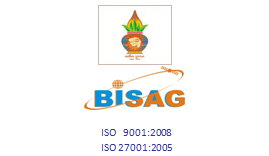
\includegraphics [scale=0.47] {Bisag.png}\\
\end{center}
\end{figure}

\begin{center}
\bf{Bhaskaracharya Institute for Space Applications \& Geo-informatics}\\
\bf{Govt.of Gujarat,Science \& Technology, Gandhinagar}\\

\end{center}
\begin{center}
Prepared By\\
\begin{tabular}{ l p{1 cm} l }
{\large \bf Arpan Chavda} & & {\large \bf Hitesh Piprotar} \\
{\bf 09BCE006} & & {\bf 09BCE054}
\end{tabular}
\\
\vspace{0.35cm}
\begin{tabular}{ l p{1 cm} l }
{\bf Internal Guide,} &  & {\bf External Guide,}\\
{\large \bf Dr. Sanjay Garg} &  & {\large \bf Mr. Miren Karamta }\\
{\bf HOD,} &  & {\bf Project Manager,}\\
{\bf Dept. of Computer Science \& Engg., } & & {\bf BISAG,}\\
{\bf Institute of Technology,} & & {\bf Gandhinagar}\\
{\bf Nirma University, Ahmedabad} & & \\
\end{tabular}
Submitted to
\end{center}
\begin{figure}[h]
\begin{center}
  % Requires \usepackage{graphicx}
  
\includegraphics [scale = 0.4] {NirmaLogo.pdf}
\end{center}
\end{figure}
%\pic{60pt}{NirmaLogo.png}\\ ~\\
\begin{center}
{\bf DEPARTMENT OF COMPUTER SCIENCE AND ENGINEERING}\\
{\bf NIRMA UNIVERSITY, AHMEDABAD-382481}\\
{\bf MAY 2013}
\end{center}

% -------------------------------------------------------------------------
\newpage
\thispagestyle{empty}
\begin{center}
%\vspace{1cm}
{\LARGE \bf DEVELOPMENT OF GNU/LINUX DISTRIBUTION}\\
{\large \bf Major Project}\\
Prepared at\\
\begin{figure}[h]
\begin{center}
  % Requires \usepackage{graphicx}
  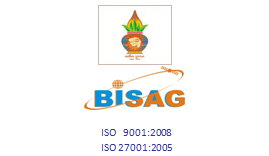
\includegraphics [scale=0.45] {Bisag.png}\\
  \end{center}
\end{figure}
\bf{Bhaskaracharya Institute for Space Applications \& Geo-informatics}\\
\bf{Govt.of Gujarat,Science \& Technology, Gandhinagar}\\
Submitted in partial fulfillment of the requirements for the degree of \\
\textbf{Bachelor of Technology in (Computer Engineering)}\\
Prepared By\\
\begin{tabular}{ l p{1 cm} l }
{\large \bf Arpan Chavda} & & {\large \bf Hitesh Piprotar} \\
{\bf 09bce006} & & {\bf 09bce054}
\end{tabular}

\vspace{0.6cm}
\begin{tabular}{ l p{1 cm} l }
{\bf Internal Guide,} &  & {\bf External Guide,}\\
{\large \bf Dr. Sanjay Garg} &  & {\large \bf Mr. Miren Karamta }\\
{\bf HOD,} &  & {\bf Project Manager,}\\
{\bf Dept. of Computer Science \& Engg., } & & {\bf BISAG,}\\
{\bf Institute of Technology,} & & {\bf Gandhinagar}\\
{\bf Nirma University, Ahmedabad} & & \\
\end{tabular}
\end{center}
\begin{figure}[h]
\begin{center}
  % Requires \usepackage{graphicx}
  
\includegraphics [scale=0.4] {NirmaLogo.pdf}
  \end{center}
\end{figure}
\begin{center}
%\pic{60pt}{NirmaLogo.png}\\ ~\\
{\bf DEPARTMENT OF COMPUTER SCIENCE AND ENGINEERING}\\
{\bf NIRMA UNIVERSITY, AHMEDABAD-382481}\\
\end{center}

% -------------------------------------------------------------------------
    \newpage
    \begin{figure}[h]
    \begin{center}
      % Requires \usepackage{graphicx}
      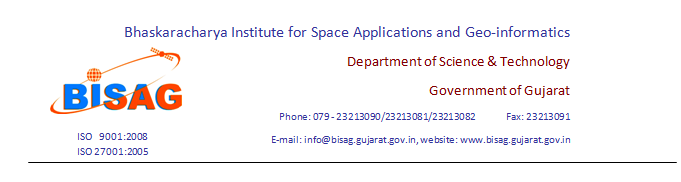
\includegraphics {BisagLogo.png}
    \end{center}
    \end{figure}

\addcontentsline{toc}{chapter}{BISAG Certificate}\label{BISAG Certificate}
\index{BISAG Certificate}
\begin{center}
{\Large \bf BISAG Certificate}\\
\end{center}
\vspace{10pt}
\noindent
This is to certify that the project report compiled by {\bf Mr Arpan Chavda(09bce006)} and {\bf Mr Hitesh Piprotar(09bce054)} students of 8th Semester B.Tech from Department Of Computer Science, Institute of Technology, Nirma University have completed their final semester project satisfactorily. To the best of our knowledge this is an original and bonafide work done by them. They have worked on “Development of GNU/Linux Distributions��, starting from January 7th, 2012 to April 24th, 2013.\\
During their tenure at this Institute, they were found to be sincere and meticulous in their work. We appreciate their enthusiasm \& dedication towards the work assigned to them.We wish them every success.
\vspace{3cm}


\noindent
\begin{tabular}{ l l l }
{\bf Mr. Miren Karamta}  & \hspace{3cm} & {\bf T. P. Singh}\\
Project Manager, &  & Director,\\
BISAG, Gandhinagar & & BISAG, Gandhinagar\\

\end{tabular}
\vspace{2cm}
\noindent

%---------------------------------
% Certificate
%---------------------------------
\newpage
\addcontentsline{toc}{chapter}{Nirma Certificate}\label{Nirma Certificate}
\index{Nirma Certificate}
\begin{center}
{\Large \bf Nirma Certificate}\\
\end{center}
\vspace{10pt}

\noindent This is to certify that the Major Project entitled {\bf "Development of GNU/Linux Distributions"} submitted by {\bf Arpan Chavda (09BCE006)} and {\bf Hitesh Piprotar (09BCE054)}, towards the partial fulfillment of the requirements for the degree of Bachelor of Technology in Computer Engineering of Nirma University, Ahmedabad is the record of work carried out by them under my supervision and guidance. In my opinion, the submitted work has reached a level required for being accepted for examination. The results embodied in this Project work, to
the best of my knowledge, haven't been submitted to any other university or institution for award of any degree or diploma.
\vspace{3cm}

\noindent
\begin{tabular}{ l l l }

{\bf Dr. Sanjay Garg}\\
Head Of Department,\\
Dept. of Computer Science \& Engg.,\\
Institute of Technology,\\
Nirma University, Ahmedabad\\

\end{tabular}
\vspace{2cm}
\noindent

\newpage
\addcontentsline{toc}{chapter}{About the company}\label{About the company}
\index{About the company}
\begin{center}
{\Large \bf About the company}\\
\end{center}
{\bf Introduction of the company}\\
\begin{figure}[h]
\begin{center}
  % Requires \usepackage{graphicx}
  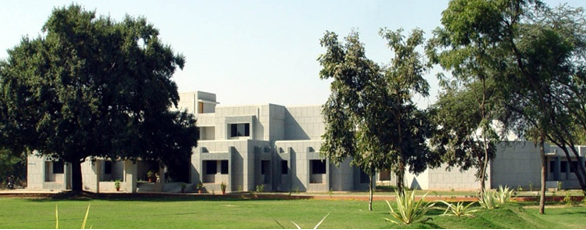
\includegraphics {Campus.png}\\
  \caption[BISAG]{BISAG}
\end{center}
\end{figure}

The applications of space technologies and geo-informatics contribute significantly towards socio-economic development of the society. Recognizing the importance and need of Space technology and geo-informatics for developmental planning purposes, the Government of Gujarat established the Bhaskaracharya Institute for Space Applications and Geo-informatics (BISAG) in the year 1997, as the State nodal agency to utilize space technology and geo-informatics for various developmental activities of the State.

Since its foundation, the Institute has experienced extensive growth in the spheres of space technology and geo-informatics. The objective with which BISAG was established is manifested in the extent of services its renders to almost all departments of the State.  Year after year the institute has been endeavoring to increase its outreach to disseminate the use of geo-informatics up to grassroots level. In this span of eleven years, BISAG has assumed multi-dimensional roles and achieved several milestones to become an integral part of the development process of the Gujarat State.
{\bf Profile}\\
BISAG’s has strengthened its role as a facility provider, a technology developer and as a facilitator for transferring technology to the grass root level.
\begin{figure}[h]
\begin{center}
  % Requires \usepackage{graphicx}
  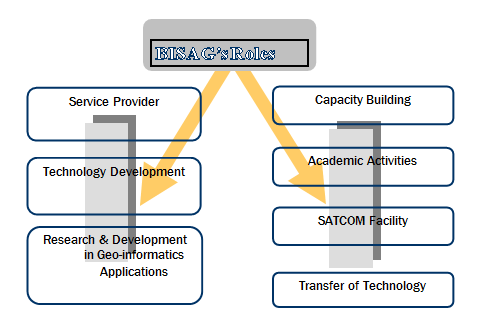
\includegraphics {BisagProfile1.png}\\
  \caption[BISAG's Role]{BISAG's Role}
\end{center}
\end{figure}
Further reinforcing its functions, BISAG has achieved ISO 9001:2008 and ISO 27001:2005 certifications for quality management and security management services respectively. This has led to an organized and systematic development of its services and outputs.\\
{\bf Activities Of BISAG}\\
BISAG’s activities are multi-fold and have expanded in a big way and focused on the following:\\

\begin{itemize}
\item {\bf Satellite Communication :} Promoting and facilitating the use of satellite broadcasting networks for distant interactive training, education and extensions

\item {\bf Remote Sensing :} Inventory mapping, developmental planning and monitoring of natural and man-made resources

\item {\bf Geo-informatics System :} Conceptualizing, creating and organizing multi-purpose common geo-spatial database for sectoral and thematic applications for various users

\item {\bf Photogrammetry :} Creation of Digital Elevation Model, Terrain characteristics, Resource planning,etc.

\item {\bf Global Navigation Satellite System :} Location based services, geo-referencing, engineering applications and research

\item {\bf Software Development :} For providing low-cost Decision Support Systems, desktop as well as web-based geo-informatics applications to users for wider usage.

\item {\bf Disaster Management :} For preparing geo-spatial information to provide necessary inputs to the Government to assess and mitigate extent of damage in the event of a disaster

\item {\bf Education, Research and Training :} For providing education, research and training facilities to promote number of end users through the Academy for Geo-informatics.

\item {\bf Value Added Services :}For providing services which can be customized as per the needs of the users.

\item {\bf Technology Transfer :} Transferring technology to a large number of end users.
\end{itemize}
{\bf Units of BISAG}\\
BISAG initially set up to carry out Space Technology applications, has evolved into an Academic Institute, a Centre for Research and Technology Innovations, a Facility Provider, a Technology Developer and a Facilitator for transferring technology to the grass root level. BISAG is the first such State Centre having such multifarious activities with ISO certification. BISAG has gradually progressed over the years and has grown into several units. Each unit focuses on specific functions and objectives to ensure efficiency in over all activities of the institute.

\begin{itemize}
\item {\bf Gujarat Satellite Communication Network (GUJSAT):} SATCOM facilitates the promotion and facilitation of the use of broadcast and teleconferencing networks for distant interactive training, education and extension.
\item {\bf Centre for Geo-Informatics Applications:} The Centre for Geo-informatics provides services for the developmental and planning activities pertaining to Agriculture, Land and Water Resources Management, Wasteland/ Watershed development, Forestry, Disaster Management, Infrastructure etc.
\item {\bf Software Development:} For wider usage of geo-spatial applications, customised software are developed by the Software Development Team. The institute has provided many indigenous software solutions in the field of Geographic Information Systems, Decision Support Systems and Image Processing.
\item {\bf Academy of Geo-informatics:}  The Academy for Geo-informatics carries out Education, Research and Training activities.
\item {\bf Disaster Management Information cell:} BISAG works closely with the Gujarat State Disaster Management Authority (GSDMA), for assessment of existing situation through integrated analysis and for planning appropriate preventive and preparatory measures, providing necessary support through data generation and analysis.
\end{itemize}

\begin{figure}[h]
\begin{center}
  % Requires \usepackage{graphicx}
  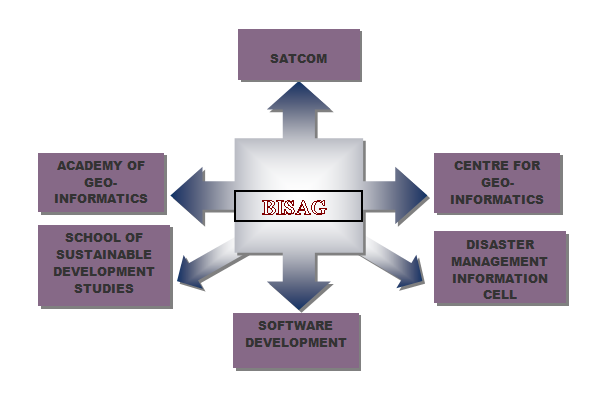
\includegraphics {BisagProfile2.png}\\
  \caption[Units of BISAG]{Units of BISAG}
\end{center}
\end{figure}
\noindent
{\bf Infrastructure Developement}\\
The growth and progress of any institute is gauged by the infrastructure it develops and possesses. BISAG has a sound infrastructure setup that has developed in tandem with the growth of the institute. Having started with one building, there are now dedicated facilities for different units.
The laboratories are equipped with state-of the art technology with latest Hardware and Software required for executing its activities. BISAG also has a rich satellite data archive, which includes Satellite data of different spatial, spectral and temporal resolutions.\\
{\bf Collaborations of BISAG...Creating A Sense Of Ownership}\\
BISAG works with almost all Government Departments and Organizations. Each of these Departments/Organization contributes in preparation of the respective projects. With strong Government support and proactive efforts on part of the staff of BISAG,
\begin{figure}[h]
\begin{center}
  % Requires \usepackage{graphicx}
  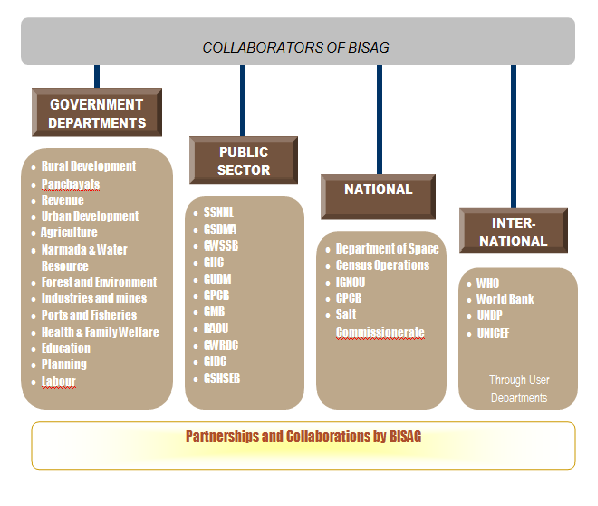
\includegraphics {BisagProfile3.png}\\
  \caption[Partnerships and Collaborations]{Partnerships and Collaborations by BISAG}
\end{center}
\end{figure}
the list of Collaborators is expanding and increasing.\\
{\bf Institutional Strengthening}
BISAG has achieved institutional strengthening through:
\begin{itemize}

\item {\bf Reinforcement of Decision Support Systems}\\
Developing customized solutions as per user requirements through partnerships and collaborations, which are affordable and easy to use. Areas of natural and manmade resources, socio-economic parameters, are being effectively addressed with the help of Geo-informatics.

\item {\bf Establishing Linkage between Government and People through GUJSAT}\\
GUJSAT facility is being constantly employed for the promotion and facilitation of the use of teleconferencing networks for distant interactive training, education and extension. Experts, leaders, specialists and professionals can conduct their programs from a central location reaching out to remote areas through two-way audio-video channel making them interactive and meaningful.

\item {\bf Developing Innovative Education Programmes}\\
Innovative educational programmes are conducted regularly through GUJSAT, allowing people residing in remote areas to have an access to good quality educational and awareness programmes.

\item {\bf Solving real life problems through Human Resource Development}\\
The institute has a young multi-disciplinary team of professionals and a continuing induction programme. Multi-nationals and IT agencies pick up the trained staff that in turn is replaced by new people. This results in availability of more and more trained manpower in the realm of space applications. Every year BISAG provides training to about 300 students in the field of Geo-informatics.


\item {\bf Creation of the multipurpose sectoral comprehensive databases for the entire state of Gujarat}\\
The institute has made efforts towards conceptualization, creation and organization of multi-purpose common digital database for sectoral / integrated decision support systems. This has provided impetus to planning and developmental activities at grass root level as well as monitoring and management potential in various disciplines like water resources, land resources, disaster management, infrastructure, urban management.
\end{itemize}
{\bf Communication}\\
The project was undertaken at BISAG, Gandhinagar and BISAG can be contacted at the following:-\\
\vspace{0.14cm}
Near Ch-0 Circle,\\
IndulalYagnikMarg,\\
Gandhinagar-Ahmedabad highway,\\
Gandhinagar-382007\\
Gujarat,India\\
\vspace{0.14cm}
Phone No:- +91 79 23213081/82/90\\


\newpage
\begin{center}
{\Large \bf Candidate’s Declaration}\\
\end{center}
We declare that final semester report entitled {\bf “DEVELOPMENT OF GNU/LINUX
DISTRIBUTIONS”} is our own work conducted under the supervision of the external guide {\bf Mr. Miren Karamta} from BISAG (Bhaskaracharya Institute for Space Applications \& Geo-informatics).We further declare that to the best of my knowledge the report for B.Tech Computer Science final semester does not contain part of the work which has been submitted for the award of Bachelor Degree either in this or any other university without proper citation.\\
\vspace{1cm}
  \\
Candidate 1’s Signature\\
Arpan Chavda\\
Student ID: 09BCE006\\
\vspace{1cm}
  \\
Candidate 2’s Signature\\
Hitesh Piprotar\\
Student ID: 09BCE054\\
\vspace{1cm}
\\
Submitted To:\\
Department Of Computer Science,\\
Institute of Technology,\\
Nirma University,\\
Ahmedabad.\\

\newpage
\index{Acknowledgements}
\addcontentsline{toc}{chapter}{Acknowledgements}
\begin{center}
{\Large \bf Acknowledgements}\\
\end{center}
\vspace{10pt}
\noindent
Gratitude is a feeling which is more eloquent than words, more tranquil than silence”.

We are grateful to {\bf T.P.Singh}, Director (BISAG) for giving us this opportunity to work the guidance of renowned people of the field of GIS also providing us with the required resources in the company.
We would like to express our endless thanks to our external guide {\bf Mr. Miren Karamta}, Project Manager at Bhaskaracharya Institute of Space Application and Geo-informatics for their sincere and dedicated guidance throughout the project development.
Also our hearty gratitude to our Head of Department and internal guide, {\bf Dr. Sanjay Garg}  for giving us encouragement and technical support on the project.

The blessings of God and our family members made the way for completion of the major project. We are very much grateful to them.

We are immensely thankful to our friends, who always stood beside and motivated me throughout this course.


\begin{flushleft}
\textbf{ Arpan Chavda}\\ \textbf{ID: 09BCE006}\\
\textbf{ Hitesh Piprotar}\\ \textbf{ID: 09BCE054}
\end{flushleft}


\newpage
% ABSTRACT
\index{Abstract}
\begin{center}
{\Large \bf Abstract}\\
\end{center}\addcontentsline{toc}{chapter}{Abstract}
\vspace{10pt}
The project named Development of GNU/Linux distribution �is designed for developers,students,programmers,coders and software engineers.This project actually contains development of two linux distributions which are free and
open source.First Distribution namely {\bf DMLinux}({\bf D}evelopers {\bf M}ono {\bf L}inux) originally forked form ubuntu is for developers.The purpose of DMLinux aims to provide all packages and all the softwares to developers 
and students who don�t have very high speed internet connection or who lives in remote area.Second distribution namely {\bf OpenGujarat} is for the students of entire gujarat students.The purpose of OpenGujarat is to provide an Operating Syatem to Gujarat students which is completely in regional language (Gujarati).



% ACKS
